\chapter{讨论}
前面我们分别描述了现有的 RNA-Seq 数据分析方法 (第 \ref{chap-intro} 章)。 
此外, 我们提出了一个通过 RNA-Seq 数据估计转录本的长度的方法 (第 \ref{chap-lenest} 章)。  
同时, 我们初步分析了 RNA-Seq 数据分布的不均匀性 (第 \ref{chap-rna-seq-nonunif} 章)。  
另外, 我们证明了通过真核生物 RNA-Seq 数据辨识基因的转录组问题是一个 NP 难问题 (第 \ref{chap-rna-seq-nphard} 章)。   
在这一章中我们对前面的内容和 RNA-Seq 数据分析方法的未来的发展方向进行讨论, 
并且对本文进行总结。 

\section{通过 RNA-Seq 数据估计转录本的长度}
在第 \ref{chap-lenest} 章的分析中我们只对单端等长读段测序数据进行了考虑, 
对于双端数据或者长度不均的读段均未作具体分析。 
在实际应用中可以只对双端数据考虑等长的在原转录本的 5' (或者 3') 端, 
或者长度不均的读段考虑等长的在原转录本的 5' (或者 3') 端, 
从而可以用第 \ref{chap-lenest} 章中的方法进行分析。 

此外, 第 \ref{chap-lenest} 章中所介绍的方法并没有考虑 RNA-Seq 
数据中读段分布受转录本序列以及转录本长度等因素造成的分布不均匀性。 
另外, 第 \ref{chap-lenest} 章中所介绍的方法也未考虑读段分布的非独立性。 
这些问题都是需要进一步继续的研究来解决的。 

\section{通过真核生物 RNA-Seq 数据估计基因的转录组}
根据第 \ref{chap-rna-seq-nphard} 章中的讨论, 
我们知道通过目前的 RNA-Seq 技术从 RNA-Seq 数据中直接估计转录组中转录本的组成在计算上是比较困难的。 
同样的问题在通过测序数据估计单体型 (haplotype) 
\cite{Li_Kim_Waterman_2004, Xing_Jordan_Sharan_2007} 时也是同样存在的 \cite{1668028}。 

随着测序技术的发展, 
RNA-PET \cite{Fullwood01042009} 技术可以对直接用来确定转录本的 5' 端和 3' 端, 
另外更长的测序读段 (例如 PacBio 研发的单分子测序技术 \cite{hybrid.rna.seq.2012})
可以帮助我们在测序数据得到后不需要使用类似第 \ref{chap-rna-seq-nphard} 
章给出的复杂的方法就能简单地直接从数据中确定转录组由哪些转录本组成。 

\section{现有 RNA-Seq 数据处理方法中存在的一些问题}
目前已有的用于 RNA-Seq 数据辨识基因的剪切异构体和估计表达量的方法 
(\ref{intro-rna-seq-tools-summary}) 仍然存在不足。 
对于真核生物 RNA-Seq 数据, 辨识基因的剪切异构体复杂度高。
此外, 当有两个转录本其中一个转录本的一端位于另一个转录本的中间时 
(图 \ref{disc-human-gene-alternative-start-1}), 
目前没有有效的方法通过 RNA-Seq 数据对这两个转录本进行区分。
另外, 对于原核生物, 尤其是原核生物中的操纵子, 的分析方法仍然没有较规范的分析方法 
\cite{mcclure2013computational} (图 \ref{disc-bacteria-operons-1})。
同时, 估计转录本表达量时仍无系统的方法处理 RNA-Seq 数据中读段分布的不均性, 
以及转录本序列的组成带来的误差 \cite{oshlack2009transcript, jones2012new}。

\begin{figure}[!t]
\centering
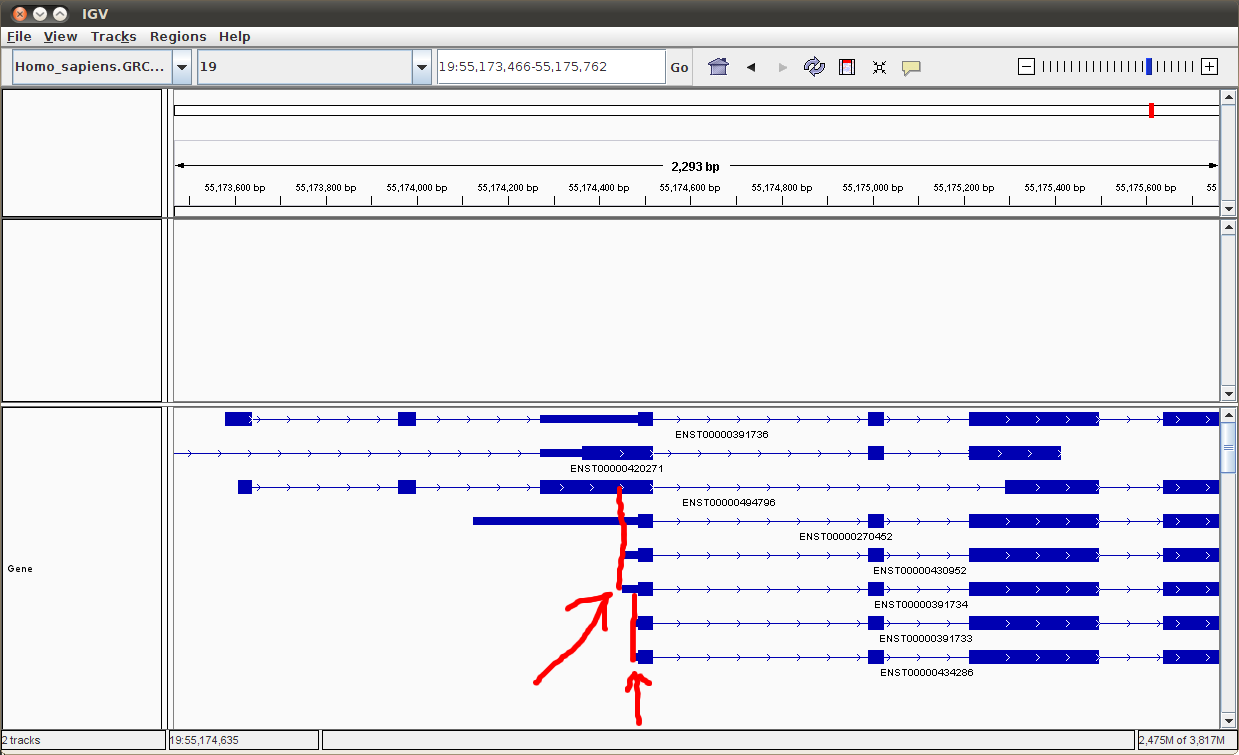
\includegraphics[width=\textwidth]{figures/disc/disc-human-gene-alternative-start-1.png}
\caption[人的基因组中出现的一个转录本的一端位于另一个转录本的中间的现象]
{人的基因组中出现的一个转录本的一端位于另一个转录本的中间的现象: 图中可见若干个基因的 5' 端位于另外的基因的中间。}
\label{disc-human-gene-alternative-start-1}
\end{figure}

\begin{figure}[!t]
\centering
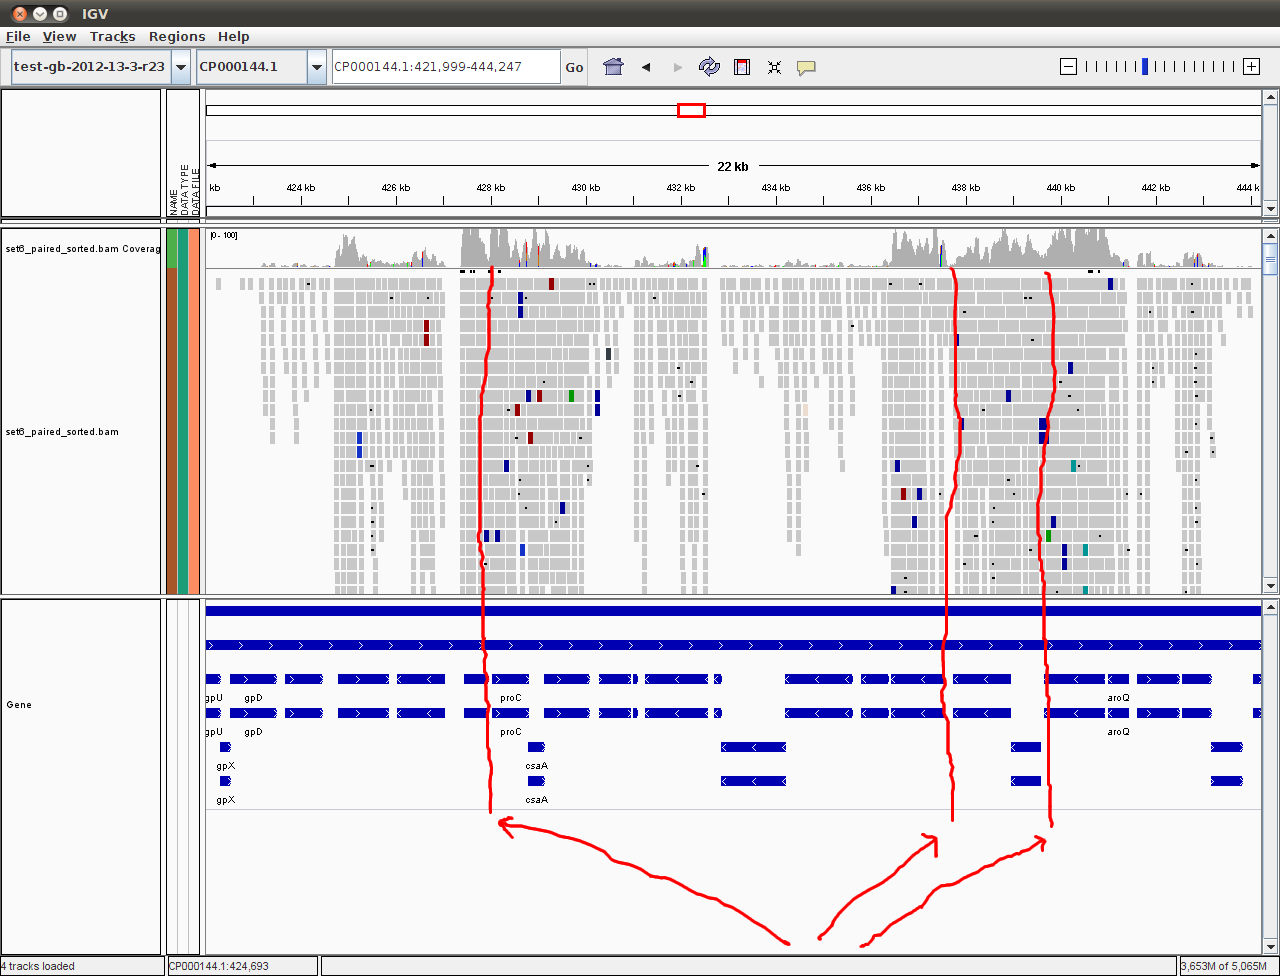
\includegraphics[width=\textwidth]{figures/disc/disc-bacteria-operons-1.png}
\caption[Giannoukos et al. 在 \onlinecite{giannoukos2012efficient} 中提供的细菌的 RNA-Seq 数据]
{Giannoukos et al. 在 \onlinecite{giannoukos2012efficient} 中提供的细菌的 RNA-Seq 数据: 
其中可以看见多个基因构成的操纵子}
\label{disc-bacteria-operons-1}
\end{figure}

\section{未来 RNA-Seq 数据的定量分析方法的工作}

\subsection{RNA-PET 测序技术} %% 序列比对, 拼装
Fullwood et al. 在 \onlinecite{Fullwood01042009} 中介绍了 RNA-PET 技术。 
通过 RNA-PET 技术我们可以对转录本的 5' 端和 3' 端的序列进行测序。 
这样我们就可以较为准确地确定转录本的 5' 端和 3' 端。 
为了处理 RNA-PET 数据, 我们需要实开发新的生物信息工具能够有效地将 RNA-PET 
数据中的读段比对到参考基因序列上。 此外, 我们还需要开发新的生物信息工具能够有效地将 RNA-PET 
数据中的读段融合到序列拼装中, 提高转录组序列拼装的质量。 

\subsection{更长的测序读段} %% 序列比对, 拼装
目前大部分 RNA-Seq 都是使用 Illumina 的平台进行测序的, 
这使得大部分的 RNA-Seq 数据都是长度小于 100 bp 的读段。 
虽然 454 的平台能够测量长度为数百 bp 的读段, 
但是 454 的平台的测序通量与 Illumina 的平台的测序通量相比较低, 
不适合通过测序的放啊对转录组进行研究。 

新的测序技术, 例如 PacBio 开发的单分子测序技术, 能够提供更长的测序读段。 
但是由于其中测序错误较多, 并且测序通量和 Illumina 的平台的测序通量相比较低, 
所以目前的做法是将 PacBio 的单分子测序技术得到的少量的长读段和 Illumina 
的平台上通过高通量测序得到的大量的短读段结合在一起进行分析 \cite{hybrid.rna.seq.2012}。 

我们需要开发出新的生物信息工具能够针对新的测序技术提供的更长的读段进行处理, 
比较重要的包括针对新的测序技术的序列比对工具和针对新的测序技术的序列拼装工具

\subsection{原核生物}
原核生物的 RNA-Seq 数据分析对于对于我们研究微生物中的基因表达是十分有意义的。 
此外, 近几年来兴起的宏转录组 (metatranscriptome) 的研究也帮助了我们对于微生物群落有了更为深入的了解
\cite{gilbert2008detection, urich2008simultaneous, gifford2010quantitative, 
helbling2011activity, mason2012metagenome, huson2011integrative, 
lesniewski2012metatranscriptome}。 

\nocite{sorek2009prokaryotic}

与真核生物不同, 原核生物中多个基因会被同时翻译到一个转录本中形成一个操纵子 
(图 \ref{e.coli.lactose.operon})。 
最近几年的研究表明 \cite{MarcGuell11272009, koide2009prevalence}, 
原核生物在不同的环境条件下在基因组的同一段区域可能产生不同的操纵子。 
通过 RNA-Seq 数据辨识原核生物操纵子也将可能成为原核生物 RNA-Seq 数据分析中的重要的一步。 

另外, 在原核生物的转录组中有大量的 rRNA (ribosomal RNA)。  
在 RNA-Seq 实验中, 
rRNA 和其他种类的 RNA (例如 mRNA) 相比起来 rRNA 含量可能超过 
90\% \cite{giannoukos2012efficient}。 
此时, rRNA 的含量会对于研究其他种类的 RNA 产生较大的负面影响。 
目前 \onlinecite{giannoukos2012efficient} 中使用了一种新的实验技术, 
可以在测序前减少样本中 rRNA 的含量。 

\begin{figure}[!t]
\centering
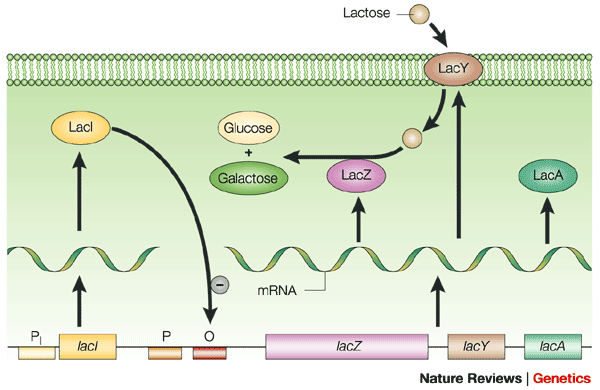
\includegraphics[width=\textwidth]{figures/disc/e-coli-lactose-operon.png}
\caption[\textit{E. coli} 中的乳糖操纵子 \cite{shuman2003art}]
{\textit{E. coli} 中的乳糖操纵子 \cite{shuman2003art}: 
基因 \textit{lacZ}, \textit{lacY}, 和 \textit{lacA} 被转录到同一个 mRNA 中}
\label{e.coli.lactose.operon}
\end{figure}

\section{总结}
本文的主要贡献在于本文提出了一个能够在没有基因注释信息的情况下通过 RNA-Seq 数据估计转录本长度的方法, 
同时证明了使用真核生物 RNA-Seq 数据通过最大似然辨识基因的剪切异构体是一个 NP 难问题。
我们期待测序技术的发展能够缓解 RNA-Seq 数据中读段分布不均匀的现象。
此外, 我们期待新的测序技术的的发展能够降低测序数据计算处理的要求, 
同时方便我们对生物问题进行研究。









